\chapter{Lecture 11}

%--- 信息 ----
\begin{center}
    讲师:王立威 \qquad
    课程时间:25.Apr.29th \qquad 
    笔记:25.June.9th
\end{center}

\bigskip

在介绍信道编码定理(Channel Coding Theorem, CCT)之前,先了解一下渐进等分性(Asymptotic Equipartition Property, AEP). 我们不加证明地使用最简单的弱大数律(WLLN) 
\begin{theorem}[弱大数律,WLLN]
    若随机变量$X,X_1,X_2,\dots,X_n,\dots$是i.i.d.的,且$\E X$存在(有界),那么对于任意$\varepsilon > 0$,有 
    \[
    \lim_{n\ra \infty}\Pr\left[
        \abs{
            \dfrac 1n \sum_{i} X_i - \E X
        } \ge \varepsilon
    \right] = 0
    \]
\end{theorem}
\begin{corollary}
    若随机变量$X,X_1,X_2,\dots,X_n,\dots$是i.i.d.的,且$\E X$存在(有界),对于任意函数$g$和$\varepsilon > 0$,有 
    \[
    \lim_{n\ra \infty}\Pr\left[
        \abs{
            \dfrac 1n \sum_{i} g(X_i) - \E g(X)
        } \ge \varepsilon
    \right] = 0
    \]
\end{corollary}
\begin{corollary}
    若离散随机变量$X,X_1,X_2,\dots,X_n,\dots$是i.i.d.的,且$\E X$存在(有界),记其分布列为$p(x)$,则对任意$\varepsilon > 0$,有 
    \[
    \lim_{n\ra \infty}\Pr\left[
        \abs{
            \dfrac 1n \sum_{i} \log\dfrac{1}{p(X_i)} - \E \log \dfrac{1}{p(X)}
        } \ge \varepsilon
    \right] = 0
    \]
\end{corollary}

我们现在考虑$X$服从Bernoulli分布,且$\Pr[X=1]=p$,仍然i.i.d.地采样出$X_1,X_2,\dots$,那么上面的推论就说明
以$\approx 1$的概率,会有 
\[
2^{-n(H(X) + \varepsilon)} \le \Pr[X_1, \dots, X_n] \le 2^{-n(H(X) - \varepsilon)}
\] 

从概率的角度,我们可以忽视余下的情况. 此后开始把上式记作如下记号
\[
\Pr[X_1, \dots, X_n] \ \dot{\approx} \ 2^{-n H(X)}
\]

我们记集合 
\[
A:= \{(x_1, x_2, \dots, x_n) : P(x_1,x_2,\dots, x_n \ \dot{\approx} \ 2^{-nH(X)})\}
\]

称$A$为\textbf{典型集}(typical set),$A$中的元素称为\textbf{典型序列}(typical sequence). 由于每个序列取到的概率是一样的,所以上面的分析导出
\begin{theorem}[AEP]
    $\abs{A} \approx 2^{nH(X)}$
\end{theorem}

当然,我们对于$(X,Y), (X_1,Y_1),\dots $i.i.d. $\sim p(x,y)$,也可以定义其联合典型集和联合典型序列。$\abs{A} \approx 2^{nH(X,Y)}$

另外,联合采样也可以看作依据似然(条件概率)分布采样,并保留性质$2^{nH(Y|X)} = 2^{nH(X,Y)} / 2^{nH(X)}$. 

这样来说,可以考虑:如果我们分别独立地按照边缘概率分布在典型集中采样(其实不强调典型集也可以,以为几乎以概率1落在典型集内)$x_1,x_2,\dots, x_n$和$y_1,y_2,\dots, y_n$. 试问将其融合得到的$(x_1,y_1), (x_2,y_2),\dots,(x_n,y_n)$也在典型集中的概率是多少?很显然是 
\[
\dfrac{2^{n H(X,Y)}}{2^{n H(X)}\cdot 2^{nH(Y)}} = \dfrac{2^{nH(Y|X)}}{2^{nH(Y)}} = 2^{-nI(X;Y)}
\]

请注意,上面的两种计算方法对应了两种理解方式!

\bigskip
另外,本节内容均是为后面铺垫。

% \begin{figure}[H]
%     \centering
%     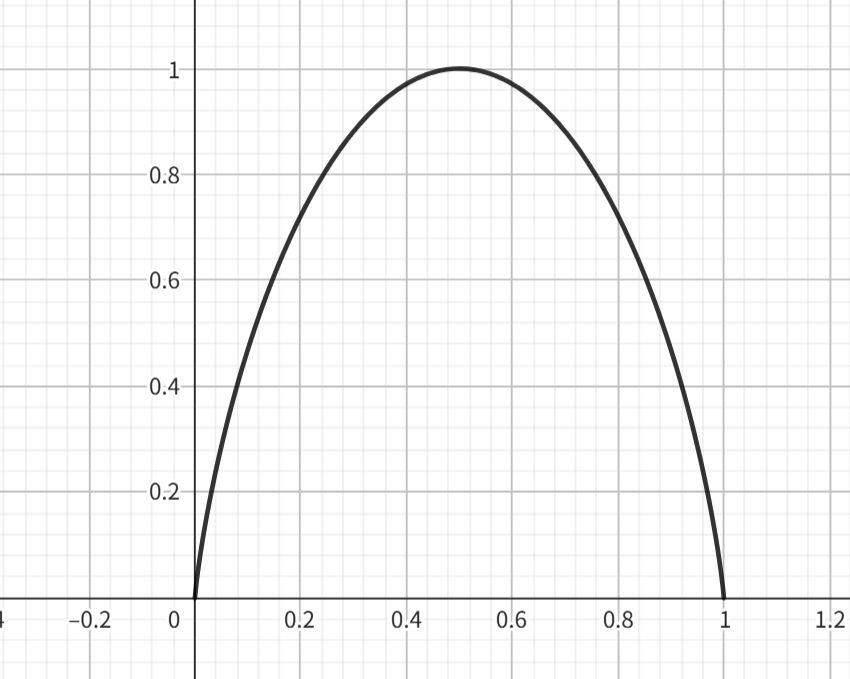
\includegraphics[width=.6\textwidth]{images/c2_1.png}
%     \caption{$H=x\log 1/x + (1-x)\log 1/(1-x)$的图像}
% \end{figure}